\section{Dataset Creation}
\label{sec:datasets}

Our work leverages two new datasets to expand the language coverage of speech technology.
In this section, we first detail how we create a labeled dataset which includes speech audio paired with corresponding text in \nummmslang{} languages (\MMS{}; \nummmshrs{} hours; \textsection\ref{sec:data-paired}). 
Second, we discuss the creation of an unlabeled dataset for which we only have audio recordings and no corresponding text.
This dataset spans \numgrnlang{} languages (\GRN{}; {\numgrnhrs} total hours; \textsection\ref{sec:data-unpaired}). 

We also use an unlabeled version of \MMS{} for pre-training and language identification. 
This spans a larger number of languages, as we can also use unlabeled audio from our data source (\MMSU{}; \nummmsulang{} languages; {\nummmsuhrs} hours). 
\autoref{fig:datasets-comp} compares the datasets to existing corpora.
A full list of the languages supported is available at \url{https://github.com/facebookresearch/fairseq/tree/main/examples/mms}.

\insertDatasetLanguageComparison

\subsection{Paired Data for \nummmslang{} Languages (\MMS{})}
\label{sec:data-paired}

We obtain speech data and transcriptions for \nummmslang{} languages by aligning New Testament texts obtained from online sources (\textsection\ref{sec:data-paired-source}) using the following steps:

\begin{enumerate}
    \item Download and preprocess both the speech audio and the text data (\textsection\ref{sec:data-preprocess}). 
    
    \item Apply a scalable alignment algorithm which can force align very long audio files with text and do this for data in 1000+ languages (\textsection\ref{sec:data-align-algo}).

        
    \item Initial Data Alignment: we train an initial alignment model using existing multilingual speech datasets covering 8K hours of data in 127 languages and use this model to align data for all languages 
    (\textsection\ref{sec:data-initial-align}).  \label{list:flowchart_step3}
    
    \item Improved Data Alignment: we train a second alignment model on the newly aligned data for which the original alignment model has high confidence and generate the alignments again. 
    The new alignment model supports 1,130 languages and 31K hours of data including the data used in step~\ref{list:flowchart_step3} (\textsection\ref{sec:data-align2}).

    \item Final data filtering: we filter the low-quality samples of each language based on a cross-validation procedure. 
    For each language, we train a monolingual ASR model on half of the aligned data to transcribe the other half of the data.  
    We retain only samples for which the transcriptions are of acceptable quality (\textsection\ref{sec:data-cross-val}).
    
    \item We partition the data into training, development and test portions (\textsection\ref{sec:data-split}).
\end{enumerate}





\subsubsection{Data Source}
\label{sec:data-paired-source}

The \MMS{} dataset is based on recordings of people reading the New Testament in different languages.
The New Testament consists of 27 books and a total of 260 chapters. 
Specifically, we obtain data from Faith Comes By Hearing\footnote{\url{https://www.faithcomesbyhearing.com/}}, goto.bible and bible.com. 
This includes the original text data as we well as the corresponding audio recording.


\paragraph{Basic Data Characteristics.}
The data sources provide 1,626 audio recordings of the New Testament in \nummmsulang{} languages, totaling \nummmsuhrs{} hours and we refer to this data as the \MMSU{} dataset.\footnote{For the audio files with no paired text, we perform VAD and segment them into smaller files.}
Out of these, both text and audio is available for 1,306 different recordings in 1,130 languages and a total of 49K hours, which we focus on for \MMS{}.
For 99 languages, we have multiple recordings.
Each recording provides separate audio files for each chapter and the duration of each chapter is on average 6.7 minutes but there is significant variance, depending on the language and chapter.
Recordings are almost always single speaker which makes it well suited for building speech synthesis systems (\textsection\ref{sec:tts}).
However, speakers are often male which may introduce unwanted biases into machine learning models which we analyze below (\textsection\ref{sec:rai-gender-bias}).


\paragraph{Multiple Scripts or Dialects per Language.}
When there are multiple recordings per language, we found that some recordings differ in the used writing script, e.g., for Serbian there are recordings using the Latin script and another which uses Cyrillic.\footnote{Specifically, we measure the correlation of the character frequency distribution for all pairs of the recordings and examine recordings with a correlation lower than 0.99 further.}
Recordings can also differ in the spoken dialect, e.g., for the Poqomchi' language there are recordings with western and eastern dialects. 

Depending on the downstream task, we handle these cases differently: for language identification, we merge the different recordings regardless of writing script or dialect, for speech synthesis models, we choose one recording per dialect/script to avoid introducing additional speakers into the training data, and for automatic speech recognition, we combine all the recordings within the same script/dialect into one and treat them as different languages, e.g., srp-script:latin, srp-script:cyrillic.


\paragraph{Micro and Macro Language Distinction.}
When there is a micro and macro language distinction, then we generally keep micro languages as distinct languages. 
However, for languages which are part of benchmarks we use for evaluation, e.g., FLEURS~\citep{conneau2022fleurs}, we deviate from this policy if the respective benchmark only contains the macro language, by merging the micro languages.
For example, Azerbaijani is a macro language and \MMS{} provides data for two associated micro languages, North Azerbaijani and South Azerbaijani.
For ASR, our evaluation benchmarks also keep the same distinction and so we model both micro languages separately, however, for LID, one of our benchmarks, VoxLingua-107~\citep{valk2020voxlingua}, only contains the macro language, and therefore, for LID only, we merge both micro languages into a single macro language.



\paragraph{Recordings with Background Music.}
Some of the recordings contain background music and we refer to these as drama recordings.
In our final \MMS{} dataset, 38\% of languages are represented solely by a drama recording and 11\% have both drama recordings and recordings without background music (non-drama recordings).
For speech synthesis, we apply pre-processing to remove background music (\textsection\ref{sec:tts}).

While this data source covers a lot of languages, it requires careful curation to make it usable for building high-quality models which presents unique challenges given the large number of languages. 
We detail the steps we take in the remainder of this section.


\subsubsection{Data Pre-processing}
\label{sec:data-preprocess}


\paragraph{Speech.}
The original audio files are available in MP3 stereo format using a 22/24/44 kHz sampling rate. 
We convert all of them to a single channel and 16 kHz sampling rate. 

\paragraph{Text Normalization.}
We design a generic text normalization pipeline that works well across the languages we consider. 
First, we perform NFKC normalization and lower case all characters.\footnote{
For example, there are two ways to represent Ç (Latin C with combining cedilla): splitting it into Latin capital C and combining cedilla (NFKD), or having a single Unicode character C with cedilla.} 
NFKC normalization helps to make sure the character encoding is consistent.
Next, we remove HTML tags such as "\&gt;" or "nbsp;".
We also remove punctuation and try to perform this carefully by including characters for which we are confident that they are in fact punctuation.\footnote{We obtain an initial set of punctuation characters from the respective Unicode category.}

We noticed that some recordings have a relatively high rate of brackets in the text: 
our criteria is recordings where at least 3\% of verses contain brackets which resulted in about 50 recordings. 
We listened to a few instances of each recording to verify whether the text in the brackets is present in the audio or not. 
In many cases, we noticed that the text in the brackets was not spoken and we removed the brackets and the text within.



\subsubsection{Scalable Forced Alignment}
\label{sec:data-align-algo}

The chapter recordings from the data source can be up to 43 minutes long which cannot be directly used by current machine learning algorithms:
we use Transformer models which require large amounts of GPU memory and their computational complexity is quadratic in the input size.
We therefore segment the data into smaller units so it can be used by standard algorithms.
Forced alignment determines which parts of the audio correspond to which parts of the text.

Given this alignment, the data can be segmented in different ways.
In our case, we segment the data into individual verses which are typically a single sentence but can sometimes contain several sentences. 
The average duration of a verse is about 12 seconds.
\autoref{fig:align} illustrates how the alignments enable creating verse-level audio segments for each chapter recording. 
In this section we detail how we perform efficient forced alignment on GPUs.


\begin{figure}[t]
\centering
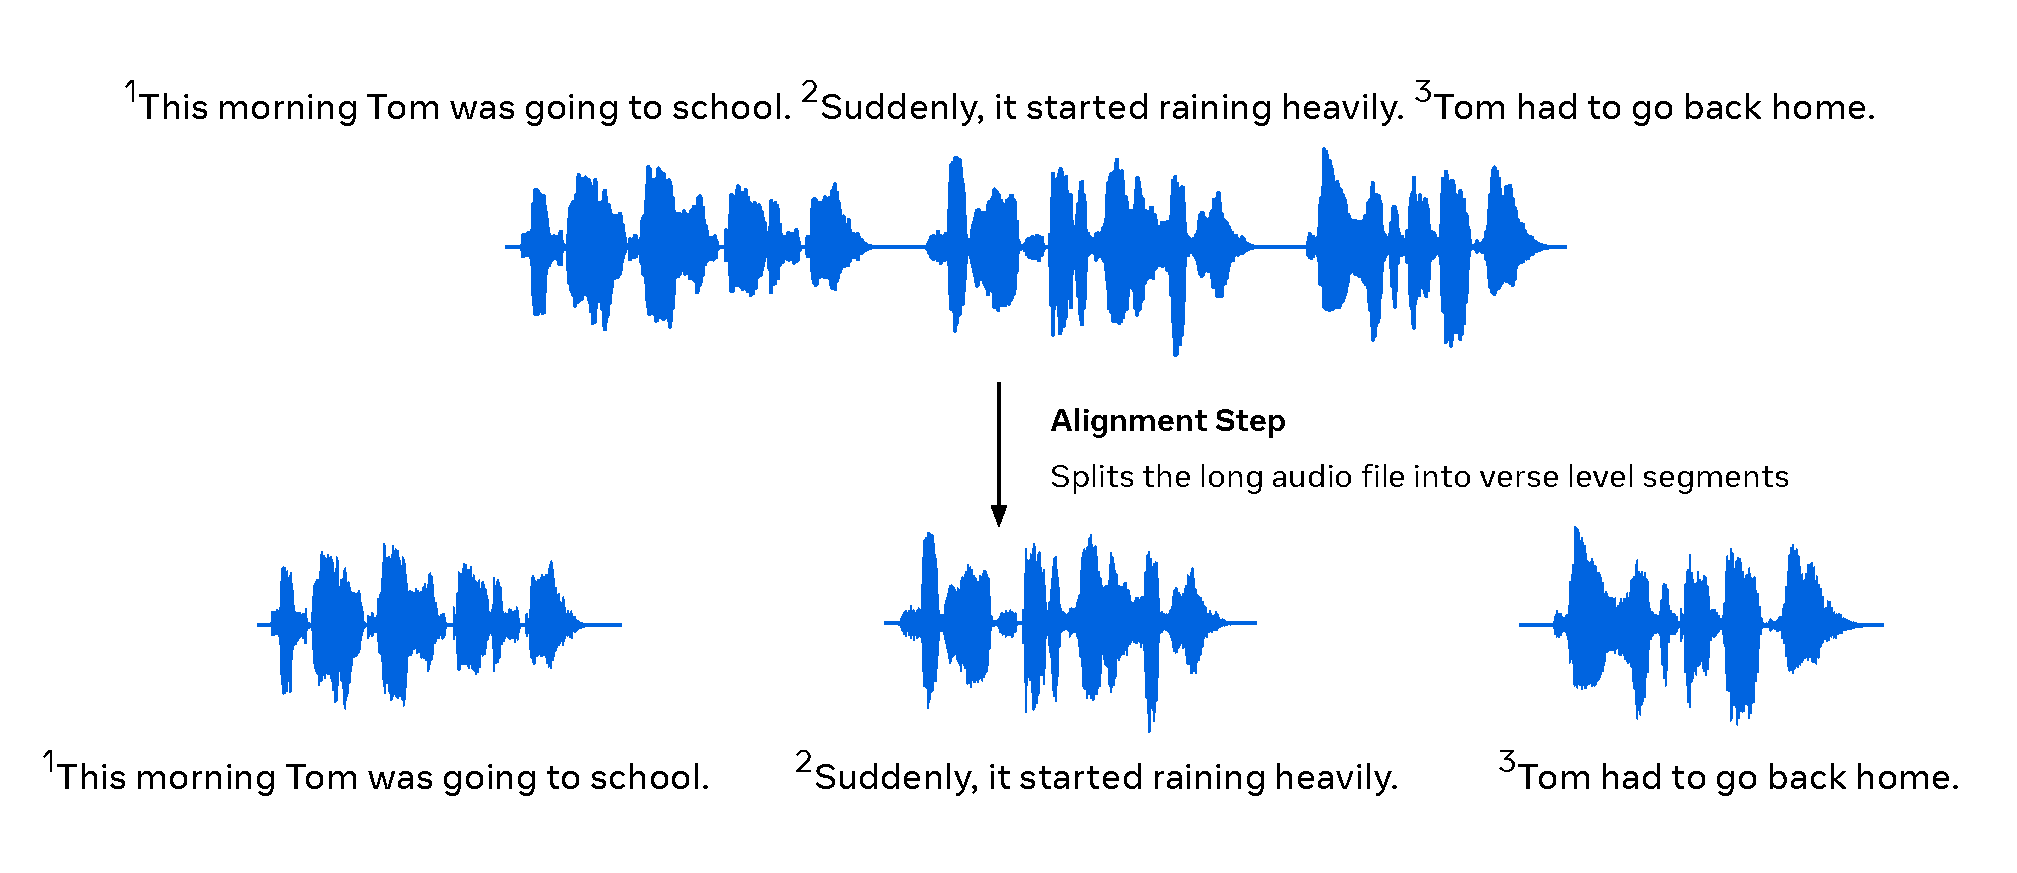
\includegraphics[width=0.9\textwidth]{images/align_all.pdf}
\caption{
\textbf{Illustration of Data Alignment.}
Forced alignment enables segmenting audio recordings and corresponding text into smaller segments that can be used to train machine learning models.}
\label{fig:align}
\end{figure}


\paragraph{Generating Posterior Probabilities.}
Forced alignment requires posterior probabilities from an acoustic model which we use for alignment (\textsection\ref{sec:data-initial-align}). 
This acoustic model is a Transformer which requires substantial amounts of memory to store activations which makes it infeasible to use for long audio files.
As a workaround, we chunk the audio files into 15 second segments, generate posterior probabilities for each audio frame using the alignment model, and then concatenate these posterior probabilities into a single matrix again.
The acoustic model is trained with Connectionist Temporal Classification (CTC;~\citealt{graves2006ctc}).


\paragraph{Forced Alignment using CTC.}
Next, we perform forced alignment which finds the most likely path in the posterior probabilities for a given input audio sequence of length $T$ and a text transcription of length $L$.
These posterior probabilities require $\mathcal{O}(T \times L)$ memory and a path will be of length $T$.
This path is computed using the Viterbi algorithm. 
There are open source libraries implementing the algorithm on CPU~\citep{ctcsegmentation,kahn2022flashlight}, however, the CPU versions are slow to run, particularly on long recordings, as we will show below.


\paragraph{Efficient Forced Alignment on GPUs.}
In order to make force alignment efficient for our purpose, we implemented a GPU version that computes the Viterbi path memory in a memory efficient way.
Storing all $\mathcal{O}(T \times L)$ forward values for the Viterbi algorithm is infeasible on GPUs due to memory constraints.
We therefore only store forward values for the current and the previous time-step and regularly transfer the computed backtracking matrices to CPU memory.
This reduces the required GPU memory to $\mathcal{O}(L)$ compared to $\mathcal{O}(T \times L)$ and enables forced alignment for very long audio sequences at high speed.
Appendix~\ref{app:align} illustrates the algorithm and an implementation is available as part of TorchAudio~\citep{yang2021torchaudio}.\footnote{\url{https://github.com/pytorch/audio}} 

\insertForceAlignBenchmark

\autoref{fig:results_fa_benchamrk} shows that the forced alignment implementation scales much better to longer sequences than CPU alternatives such as ctc-segmentation~\citep{ctcsegmentation}, a popular segmentation library used in ESPNet~\citep{watanabe2018espnet}, SpeechBrain~\citep{speechbrain} and Flashlight~\citep{kahn2022flashlight}. 
 


\paragraph{Robust Alignment for Noisy Transcripts.}
For many recordings, speakers introduce the chapter name and the version of the New Testament before reading the first verse, however, the corresponding text does not contain this information.
This is problematic for forced alignment because the algorithm will still try to align the beginning of the audio to the text which can result in incorrect alignments.
Another challenge is that numbers are generally spelled as digits in the text whereas our alignment model is trained on existing corpora which follow common practice of spelling numbers out fully (\textsection\ref{sec:data-initial-align}).
Spelling numbers out requires language-specific and hand-crafted tooling which is not available for the \nummmslang{} languages we consider.

\insertStarPlots 

To enable robust alignment in both cases, we introduce a star token ($\Star$;~\citealt{pratap2022star, cai2022wctc}) to which audio segments can be mapped if there is no good alternative in the text.\footnote{This is different from an OOV token or silence token in an HMM topology, which model a certain type of acoustic behavior and are independent from other in-vocabulary tokens.}
We insert $\Star$ at the beginning of the text data of each chapter and replace numerical digits with $\Star$ throughout. 
The posterior probability for this token is set to one.
After alignment, we add back the original digits and the subsequent data filtering often removes segments where the audio contains additional information not present in the aligned text (\textsection\ref{sec:data-cross-val}).
\autoref{fig:star_token} illustrates how adding the $\Star$ token helps to improve alignment when the paired text does not cover the beginning of the audio.



\subsubsection{Initial Data Alignment}
\label{sec:data-initial-align}

\paragraph{Acoustic Model.}
To perform the forced alignment, prior work typically uses acoustic models trained on data in the same language.
For example, for the eight languages of the MLS dataset~\cite{pratap2020mls} the authors used acoustic models trained on existing data for these languages.
However, our setting includes many languages for which no datasets or acoustic models exist.
We therefore train a multilingual acoustic model on FLEURS~\citep{conneau2022fleurs} and CommonVoice 8.0~\citep{ardila2019common} to learn a shared representation across languages which we hope to generalize to unseen languages. 
The multilingual model is based on fine-tuning XLS-R~\citep{babu22_interspeech} using a total 8K hours of data covering 127 languages.

\insertUromanXsampaExamples

\paragraph{Text Encoding.}
The text data is represented using the uroman transliteration tool~\citep{hermjakob-etal-2018-box}
which maps different writing scripts to a common Latin script representation.\footnote{\url{https://www.isi.edu/~ulf/uroman.html}}
This is done using character descriptions based on Unicode tables and a large number of additional heuristics and it has language-specific romanization rules for some languages.
Prior work~\citep{black2019cmu} used Unitran~\citep{yoon-etal-2007-multilingual,qian-etal-2010-python,black2019cmu} which converts UTF-8 encoded text into a phonetic transcription in either WorldBet~\citep{hieronymus1993ascii} or X-SAMPA~\citep{wells_1995}. 

Inspired by~\citet{black2019cmu}, we initially investigated X-SAMPA but found that uroman led to similar quality results and we decided to use uroman since it is easier to interpret compared to International Phonetic Alphabet (IPA) based symbols generated by Unitran. 
\autoref{tab:data-ex-uroman-xsampa} shows some example outputs from uroman. 
We lowercase all the letters of the uroman output and retain only \textit{a} to \textit{z} characters as well as the apostrophe character to train acoustic models for forced alignment (\autoref{sec:data-align-algo}).

% \ma{TODO [low pri]: show experiment demonstrating that our 127-lang multilingual alignment model can generalize to unseen languages. 
% Train the same model on ~120 languages, perform initial alignment step, train ASR models and compare to ASR models trained on data aligned by 127-lang alignment model.}



\subsubsection{Improved Data Alignment}
\label{sec:data-align2}

To improve the alignments, we use a subset of good-quality samples to train a new alignment model.
Samples are selected based on a score which is the length-normalized difference between the probability of the forced alignment path $P(Y^{aligned} \mid X)$ and the probability of greedy decoding from the alignment model $P(Y^{greedy} \mid X)$.  
The former is constrained by the text used in the alignment and the latter is unconstrained. 
A large difference between these two quantities may indicate that the alignment is incorrect.\footnote{It may also indicate that the alignment model is of poor quality but in practice we found that the metric identifies many incorrect alignments.}
Concretely, the score is 
\begin{equation}
    \centering
      \frac{1}{T} \log P(Y^{aligned} \mid X) - \log P(Y^{greedy} \mid X)
\end{equation}
where $T$ is the length of the audio.
The score can vary from $-\inf$, indicating low quality samples, to $0$, indicating high quality samples. 
After manual inspection of sample quality and their corresponding score for several languages, we select $-0.2$ as the threshold and choose samples with scores greater than this threshold.
The improved alignment model is trained on a total of 31K hours in 1,130 languages which includes the data we used for the initial alignment model.\footnote{This model is available at \url{https://github.com/facebookresearch/fairseq/tree/main/examples/mms}}
We use this new model to re-generate verse level alignments for our data. 



\subsubsection{Final Data Filtering}
\label{sec:data-cross-val}

After generating the improved alignments, we noticed that some samples are still of low quality.
Some recordings are not entirely faithful to the text and speakers sometimes add their own interpretation or paraphrase parts of the text. 
This will negatively impact ASR and TTS models trained on the data and we therefore perform a final data filtering step to improve data quality as much as possible.

We we train monolingual ASR models on half of the the aligned samples of each recording, measure performance on the remaining half and remove samples which have a character error rate (CER) in excess of 10\%. 
This removes about 1.7\% of all samples across all languages. 

High CER may be due to low quality samples in either half of the data, that is the training data of the ASR model or the data being evaluated. 
To help ensure we use recordings that are generally of good quality, we remove 3837 recordings which have CER in excess of 5\% on the developmet set.
We retain a total of 1,239 recordings covering 1,107 languages.

\subsubsection{Creating train/dev/test splits}
\label{sec:data-split}

\insertMMSHours

The recordings often contain only a single speaker which makes it challenging to measure generalization performance of models trained on this data.
This is why we evaluate models trained on \MMS{} data on existing benchmarks as much as possible in the remainder of this paper.
The advantage of this is that it side steps the aforementioned issues and it also enables us to better understand how the data can be useful in other domains.

However, existing benchmarks only cover a small fraction of the languages in \MMS{} and in order to be able to develop models for all languages, we split the aligned recordings into train/dev/test splits.
We aim to make the content of the splits as disjoint from each other as possible and use a similar split across different recordings.
To do so, we try to use different books for each split and use the same books for each split across recordings and languages as much as possible.

Concretely, we use the book Mark (MRK) as development set, the book John (JHN) as test set and the remaining books for training. 
For the 147 recordings where not all 260 chapters are available, we deviate from this and make a best effort split by books depending on which books are available in the respective recording.
In this case, we aim to have at least 10\% of all available data in the development set and the test set each, or at most two hours of data in each set, whichever is less.

The final dataset contains \nummmshrs{} hours of paired speech data where we use 36.8K hours for training (82.3\%), 3.5K hours for development (7.8\%) and 4.4K hours for testing (9.9\%).
For each language, the train split contains an average of 32 hours (stddev=19), the dev split contains an average of 3.1 hours (stddev=1.8) and test split an average of 3.9 hours (stddev=2.3).
\autoref{fig:data-mmshrs} shows the data distribution across languages.




\subsection{Unpaired Data for \numgrnlang{} Languages (\GRN)}
\label{sec:data-unpaired}

\paragraph{Data Source.}
The data source for this dataset is Global Recordings Network which provides recordings of Bible stories, evangelistic messages, scripture readings, and songs in more than 6,255 languages and dialects.\footnote{\url{https://globalrecordings.net/}}
The audio files are not accompanied by a corresponding text transcription but the source makes clear which language is being spoken.
We group the data by language, combining  dialects of the same language resulting in a total of 3,860 languages and 9,345 hours of audio.

\insertGRNHours

\paragraph{Pre-processing.}

We convert the audio files to single channel and a sample rate of 16kHz. 
Next, we use inaSpeechSegmenter~\citep{ddoukhanmirex2018}, a CNN-based audio segmentation model, to  identify segments of speech, music, noise and silence in the audio. 
If two segments of speech are separated by intermediate segments containing music or noise, then we consider joining these segments if the intermediate segment is no longer than 20\% of all segments together. 
This is to build samples that are of longer duration and still contain mostly speech.
The remaining non-speech segments are discarded.

Next, we randomly split the speech segments into portions of between 5.5 and 30 seconds. 
This makes the data usable for training downstream models and creates a length distribution of the samples that is in line with other datasets such as FLEURS where the average sample length is about 12 seconds.

\paragraph{Dataset Split.}
Finally, we split the samples of each language randomly into 80\% training data, 10\% development data, and 10\% test data. 
We also remove 51 languages for which we have less than 5 minutes of training data to ensure we have sufficient data to train models.
The final dataset comprises a total of \numgrnhrs{} hours of data in \numgrnlang{} languages.
The training portion is 6.2K hours and there are 770 hours for the valid and test sets each.
For each language, the train set contains an average of 97 minutes (stddev=177.4), and the dev/test sets contain an average of 12.1 minutes (stddev=22.3).
\autoref{fig:data-grnhrs} shows the data distribution across languages.



\subsection{Comparison to Existing Broad Coverage Approaches and Other Datasets}

In this section, we present a comparison to two related studies which aimed to expand speech technology to many languages.
The CMU Wilderness project~\citep{black2019cmu} also used New Testament data to build speech synthesis models for 699 languages (\textsection\ref{sec:data-comp-cmu}) and ASR-2K~\citep{li2022asr2k} focused on automatic speech recognition for nearly two thousand languages (\textsection\ref{sec:data-comp-asr2k}).
Finally, we assess the viability of the new data for building machine learning models by comparing the performance of ASR models trained on \MMS{} to models trained on an existing dataset in an out-of-domain setting (\textsection\ref{sec:data-compdata}).


\subsubsection{CMU Wilderness Dataset}
\label{sec:data-comp-cmu}

The most comparable prior work is the CMU Wilderness project which used data from similar sources~\citep{black2019cmu}. 
To better understand how our data creation process compares to their method, we conduct a best effort side-by-side reproduction of their process and use the resulting data to train monolingual ASR models under the same settings.\footnote{We reproduced the data by following the steps outlined at \url{https://github.com/festvox/datasets-CMU_Wilderness}}

To compare the effectiveness of their data creation method to ours (\textsection\ref{sec:data-paired}), we take the original data from our data source and apply either our protocol or the protocol of \citet{black2019cmu}.
For languages where multiple recordings exist, we only use the recordings used in the CMU Wilderness dataset to enable a better comparison.
Next, we use the resulting data to fine-tune XLS-R models~\citep{babu22_interspeech} for monolingual ASR and then measure accuracy in terms of character error rate on the FLEURS dev set.

\autoref{fig:data-compare-cmu} shows that the \MMS{} data preparation process results in better quality ASR models compared to CMU Wilderness with improvements between 2.1\%-4.7\% CER, depending on the language.
Our alignment procedure also retains a much larger amount of the training data compared to the CMU Wilderness protocol:
for Telugu, there are 26.5 hours of data, \MMS{} retains 26.2 hours compared to 11.1 hours for the CMU Wilderness process.
For English, we start with 17.3 hours, \MMS{} retains 17 hours vs. 10.6 hours for CMU Wilderness. 

\insertComparisonWithOtherDatasets



\subsubsection{ASR-2K}
\label{sec:data-comp-asr2k}

The most comparable multilingual ASR work to ours is ASR-2K~\citep{li2022asr2k} which covers 1,909 languages. 
Their approach is based on mapping the output of an eight language multilingual model to appropriate phonemes for the language of interest. 
In contrast, \MMS{} has actual paired speech and text data.

ASR-2K reports average character error rate (CER) on 34 languages of Common Voice 6.0 and uses a language model for decoding. 
\MMS{} covers 22 out of these 34 languages and we use it to train monolingual ASR models without language models.
The monolingual models trained on {\MMS} dataset obtain an average CER of 9.6 on 22 languages.
ASR-2K reports CER 50.9 on 34 languages.
While not a like for like comparison, this difference suggest that \MMS{} enables higher quality ASR models.
We stress that this is a best effort comparison and does not enable strong conclusions.\footnote{We could not obtain a per-language break down of the ASR-2K results.}


\subsubsection{Other Existing Datasets}
\label{sec:data-compdata}

The \MMS{} covers a large number of languages but it also has potential downsides:
it is both from a particular narrow domain and most recordings are from a single speaker. 
This may lead to poor performance on other domains or when the systems are applied to unseen speakers.

To get a better sense of both issues, we train monolingual ASR models by finetuning XLSR~\citep{babu22_interspeech} on \MMS{} and evaluate these models on the FLEURS benchmark.
For comparison, we train another set of ASR models on labeled data from Common Voice which is an existing dataset and does not have the aforementioned downsides: the domain is general and the data contains multiple speakers. 
We control the amount of training data of both datasets by using exactly ten hours of training data and one hour of development data from both datasets.

\autoref{fig:compare-cv} shows that models trained on CommonVoice perform better on 18 languages of FLEURS (average CER 9.3 vs. 12.2) but the models \MMS{} still enable good performance.\footnote{Spanish (spa), Catalan (cat), Polish (pol), German (deu), Portoguese (por), Russian (rus), Ukrainian (ukr), Turkish (tur), Swahili (swh), French (fra), Dutch (nld), Farsi (fas), English (eng), Welsh (cym), Luganda (lug), Arabic (ara), Tamil (tam), Thai (tha).}
This is despite the fact that \MMS{} utterances are often from a single speaker and are from a very narrow domain.
While there is certainly higher quality data for head languages, this result suggests that the quality of the \MMS{} data can enable high quality speech systems for a large number of other languages.



